	\subsubsection*{Description}
	Scalability is an essential aspect of a system and is the ability of a system to be easily enlarged in order to accommodate a growing amount of work.
	\subsubsection*{Justification}
	 As the Buzz System should allow for more than a million concurrent users, the system must be able to handle that large number without breaking down or reducing performance.
	\subsubsection*{Mechanism}
		\begin{enumerate}
			\item Strategy:\\\\
			Scalability can be achieved by:
			\begin{itemize}
			\item Clustering: using more resources by running many instances of the application over a cluster of servers or instances.
			
			\item Efficient use of storage: data storage can be efficiently used through compression of the data (reducing data size to make room for more) paging (ensuring that primary storage is used only for more crucial data) as well as de-fragmentation (organizing the data into continuous fragments and free more storage space).
			by ensuring that no data duplications occur, storage space can be conserved, thus the load on system resources will be reduced.
			\item Efficient persistence: through indexing and query optimization, the amount of system power used to persist a database will be reduced, as data retrieval will be quicker and costly queries will be done without, thus also reducing system load. In addition, connections can be grouped and accessed via a central channel in order to aid persistent storage to the database.
			
			\item Load Balancing: by spreading the systems load across time or across resources the load on the system can be distributed, therefore no system resource will be heavily strained. In the case that the limit for a server has been reached, a new instance or so will have to be created in order to handle the number of increasing requests. On the other hand, if the usage of a server is way below the capacity, the number of instances will have to be reduced.
			
			\item Caching: to ensure no duplication or repeated retrieval of frequent objects or queries; a separate module can facilitate caching; thus system resources will not be used up unnecessarily.
			 \end{itemize}
			\item Architectural Pattern(s):
			\begin{itemize}
			\item Blackboard Architectural Pattern
				\begin{itemize}
					\item This pattern functions by providing a framework for a systems that need to integrate varying, large specialized modules. It entails the use of three components, namely a knowledge source, a control as well as a blackboard in order to facilitate the distributed solving of problems in a system wherein there is no defined process to solve these problems. This pattern is in itself scalable, through its distributed architecture, and as such scalability can be easily achieved across a grid of processors.				
			\end{itemize}
			 \end{itemize}
			 
			 \begin{itemize}
			\item Master-Slave Architecture Pattern
				\begin{itemize}
					\item This pattern functions by splitting independent tasks over a number of independent processing grid slaves; wherein the slaves do the main work and the master manages the entire process. This allows for parallel processing, wherein each slave simultaneously performs a system operation and the results of each operation are later merged.
				 \end{itemize}
			 \end{itemize} 
		\end{enumerate}
		
		
\pagebreak	
\begin{itemize}
	\item Aspects of the Scalability discussed above can be seen as an illustration in Figure \ref{fig:scalability} below.
	\begin{figure}[H]
		\centering
		\fbox{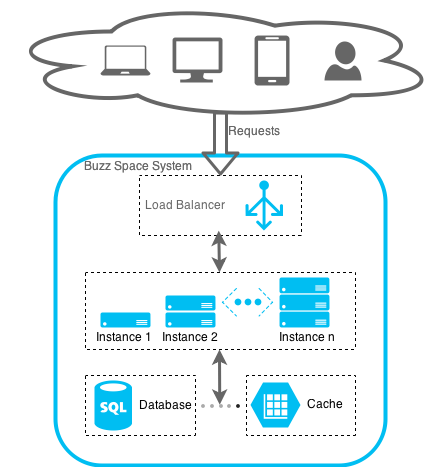
\includegraphics[width=1.0\textwidth]{Scalability}}
		\caption{How the system architecture can be set-up to allow many concurrent connections.}
		\label{fig:scalability}
	\end{figure}
\end{itemize}